% =====================================================================
%  Introduction to Neuroscience — Session 9
%  Neural signalling III: the action potential
%  Reading: Bear, Connors & Paradiso, Ch. 4; Rieke, Warland, de Ruyter van
%  Steveninck & Bialek (1997), Spikes: Exploring the Neural Code, Ch. 1
%  Rakesh Sengupta, SIAS, Krea University
% ---------------------------------------------------------------------
%  ACCESSIBLE "at a glance" format, as in Session 7 (v2): one bold headline
%  per slide (\glance), at most three bullets, fixed ion colours, a one-page
%  picture at start and end, a "So far" recap after each section.
%  Includes a short bridge from Session 7, so it also works if Session 8 is cut.
%  Companion: NEUR_S09_activity_booklet. Session number: \sessnum (preamble).
%  SPIKE LAB (jsPsych, runs in any browser, saves nothing):
%    served from this repository: labs/spike-lab/ (see \lablink below).
%    Change \lablink and \lablinkshown below if it lives elsewhere;
%    the QR codes update themselves.
%  All voltage traces are computed from the Hodgkin-Huxley (1952) model,
%  the same model Spike Lab runs (data.tex).
%  Build: pdflatex twice. Speaker notes: uncomment \setbeameroption.
% =====================================================================
\documentclass[aspectratio=169,11pt]{beamer}
% \setbeameroption{show notes on second screen=right}

\usepackage[T1]{fontenc}
\usepackage[utf8]{inputenc}
\usepackage{helvet}
\usepackage{graphicx}
\usepackage{tikz}
\usetikzlibrary{arrows.meta,positioning,shapes.geometric,calc}
\usepackage{pgfplots}
\pgfplotsset{compat=1.17}
\usepackage{booktabs}
\usepackage{array}
\usepackage{tcolorbox}
\tcbuselibrary{skins}
\usepackage{ragged2e}
\usepackage{qrcode}
\usepackage{url}
\urlstyle{sf}

% ------------------------------ THEME --------------------------------
\definecolor{kprimary}{HTML}{1F3A5F}  % deep navy
\definecolor{kaccent}{HTML}{B85A0E}   % saffron, darkened for contrast
\definecolor{kgreen}{HTML}{23665A}
\definecolor{kred}{HTML}{A12F24}
\definecolor{kpale}{HTML}{F7F3EA}
\definecolor{kgrey}{HTML}{4B5563}

\usetheme{default}
\usefonttheme{professionalfonts}
\setbeamertemplate{navigation symbols}{}
\setbeamercolor{normal text}{fg=black!88}
\setbeamercolor{structure}{fg=kprimary}
\setbeamercolor{frametitle}{fg=white,bg=kprimary}
\setbeamercolor{title}{fg=kprimary}
\setbeamercolor{subtitle}{fg=kaccent}
\setbeamerfont{frametitle}{series=\bfseries,size=\large}
\setbeamerfont{title}{series=\bfseries,size=\huge}
\setbeamerfont{subtitle}{size=\large}
\setbeamertemplate{itemize item}{\color{kaccent}$\blacktriangleright$}
\setbeamertemplate{itemize subitem}{\color{kgrey}--}
\setbeamertemplate{enumerate item}{\color{kprimary}\bfseries\insertenumlabel.}
\addtobeamertemplate{frame begin}{}{\RaggedRight}
\hyphenpenalty=10000 \exhyphenpenalty=10000 \tolerance=9000 \emergencystretch=3em

% slide-type label on the right of the title bar (passed as the frame subtitle)
\makeatletter
\setbeamertemplate{frametitle}{%
  \nointerlineskip
  \begin{beamercolorbox}[wd=\paperwidth,ht=2.7ex,dp=1.2ex,leftskip=1em,rightskip=1em]{frametitle}
    \usebeamerfont{frametitle}\insertframetitle\hfill
    \ifx\beamer@framesubtitle\@empty\else\insertframesubtitle\fi
  \end{beamercolorbox}}
\makeatother
\newcommand{\tagpill}[3]{{\normalfont\footnotesize\setlength{\fboxsep}{2.5pt}\colorbox{#1}{\textcolor{#2}{\bfseries #3}}}}
\newcommand{\tPlan}{\tagpill{white}{kprimary}{PLAN}}
\newcommand{\tIdea}{\tagpill{white}{kprimary}{IDEA}}
\newcommand{\tStudy}{\tagpill{white}{kgreen}{STUDY}}
\newcommand{\tThink}{\tagpill{white}{kaccent}{THINK}}
\newcommand{\tAct}{\tagpill{kaccent}{white}{ACTIVITY}}
\newcommand{\tAns}{\tagpill{kgreen}{white}{ANSWERS}}
\newcommand{\tCaution}{\tagpill{kred}{white}{CAUTION}}
\newcommand{\tRef}{\tagpill{white}{kgrey}{REFERENCE}}
\newcommand{\tLab}{\tagpill{kgreen}{white}{SPIKE LAB}}
\newcommand{\sessnum}{9}  % change here if the session is renumbered

% roadmap in the footer: the current part is bold, saffron and marked with a triangle
\newcommand{\rmitem}[2]{\ifnum\value{section}=#1{\color{kaccent}\bfseries$\blacktriangleright$\,#2}\else{\color{kgrey}#2}\fi}
\setbeamertemplate{footline}{%
  \hbox{\begin{beamercolorbox}[wd=\paperwidth,ht=2.6ex,dp=1.1ex,leftskip=1em,rightskip=1em]{}
    \scriptsize \rmitem{1}{Opening}\quad\rmitem{2}{1 The spike}\quad\rmitem{3}{2 The doors}\quad\rmitem{4}{3 The pause}\quad\rmitem{5}{4 The code}\quad\rmitem{6}{Wrap-up}
    \hfill{\color{kgrey}Session \sessnum\ \,$\cdot$\, \insertframenumber/\inserttotalframenumber}
  \end{beamercolorbox}}}

% big roadmap for section dividers
\newcommand{\roadmapbig}{%
  
\begin{tikzpicture}[rb/.style={draw=kpale,rounded corners=3pt,minimum width=2.05cm,minimum height=0.95cm,font=\small,align=center,text=kpale}]
    \foreach \i/\t in {1/{Opening},2/{1 The\\spike},3/{2 The\\doors},4/{3 The\\pause},5/{4 The\\code},6/{Wrap-up}}{
      \ifnum\value{section}=\i
        \node[rb,fill=kaccent,draw=kaccent,text=white,font=\small\bfseries] (r\i) at (\i*2.25,0) {\t};
        \node[font=\small\bfseries,text=white] at (\i*2.25,-0.85) {you are here};
      \else
        \node[rb] (r\i) at (\i*2.25,0) {\t};
      \fi}
  \end{tikzpicture}}

\AtBeginSection[]{%
  \begin{frame}[plain]
    \begin{tikzpicture}[remember picture,overlay]
      \fill[kprimary] (current page.south west) rectangle (current page.north east);
    \end{tikzpicture}
    \vspace{1.2cm}
    {\color{white}\Huge\bfseries \insertsectionhead\par}
    \vspace{0.6em}
    {\color{kpale}\large \sectionsub\par}
    \vspace{1.6em}
    \roadmapbig
  \end{frame}}
\newcommand{\sectionsub}{}

% ---------- helpers ----------
\newcommand{\imgslot}[4]{%
  \IfFileExists{images/#1}%
    {\includegraphics[width=#2,height=#3,keepaspectratio]{images/#1}}%
    {\begin{tikzpicture}
       \node[draw=kgrey,dashed,rounded corners,fill=kpale,
             minimum width=#2,minimum height=#3,
             text width=\dimexpr#2-10pt\relax,align=center,font=\footnotesize\color{kgrey}]
             {\textbf{\color{kprimary}Image slot}\\[2pt] #4\\[3pt] \texttt{\scriptsize images/\detokenize{#1}}};
     \end{tikzpicture}}}
\newcommand{\hl}[1]{\textcolor{kaccent}{\textbf{#1}}}
\newcommand{\src}[1]{{\footnotesize\color{kgrey}(#1)}}
\newtcolorbox{askbox}[1][]{enhanced,colback=kaccent!8,colframe=kaccent,halign=flush left,halign title=flush left,
  arc=2mm,boxrule=0.9pt,left=7pt,right=7pt,top=5pt,bottom=5pt,
  title={\bfseries Think (writing or passing is fine)},fonttitle=\small,coltitle=white,#1}
\newtcolorbox{factbox}[1][]{enhanced,colback=kprimary!5,colframe=kprimary,halign=flush left,halign title=flush left,
  arc=2mm,boxrule=0.9pt,left=7pt,right=7pt,top=5pt,bottom=5pt,fonttitle=\small\bfseries,coltitle=white,#1}
\newtcolorbox{donebox}[1][]{enhanced,colback=kgreen!7,colframe=kgreen,halign=flush left,halign title=flush left,
  arc=2mm,boxrule=0.9pt,left=7pt,right=7pt,top=4pt,bottom=4pt,
  title={\bfseries You are done when},fonttitle=\small,coltitle=white,#1}
\newcommand{\infopill}[2]{{\setlength{\fboxsep}{4pt}\fcolorbox{kaccent}{kaccent!8}{\small\textbf{#1:}\ #2}}}
\newcommand{\actinfo}[3]{\noindent\infopill{Time}{#1}\hspace{0.5em}\infopill{Who}{#2}\hspace{0.5em}\infopill{Where}{#3}\par\medskip}

\tikzset{
  tile/.style={draw=#1,fill=#1!8,rounded corners=3pt,align=left,font=\small},
  grp/.style={draw=#1,fill=#1!10,rounded corners=3pt,font=\small\bfseries,minimum width=2.6cm,minimum height=1.0cm,align=center},
  card/.style={draw=kaccent,fill=kaccent!8,rounded corners=3pt,minimum height=1.3cm,text width=3.9cm,align=left,font=\small}}

% ---------- at-a-glance additions (v2) ----------
\newcommand{\cb}{$\square$\ }
% Ion colours: the same everywhere in the deck and booklet. Ions are always labelled too, so colour is never the only cue.
\definecolor{cNa}{HTML}{B85A0E}  % sodium: saffron
\definecolor{cK}{HTML}{6A3D9A}   % potassium: purple
\definecolor{cCl}{HTML}{23665A}  % chloride: green
\definecolor{cCa}{HTML}{A12F24}  % calcium: red
\newcommand{\Na}{\textcolor{cNa}{\textbf{Na$^{+}$}}}
\newcommand{\K}{\textcolor{cK}{\textbf{K$^{+}$}}}
\newcommand{\Cl}{\textcolor{cCl}{\textbf{Cl$^{-}$}}}
\newcommand{\Ca}{\textcolor{cCa}{\textbf{Ca$^{2+}$}}}

% The one line to remember, at the top of every content slide
\newcommand{\glance}[1]{%
  \begin{tcolorbox}[enhanced,colback=kpale,colframe=kpale,borderline west={3pt}{0pt}{kaccent},arc=0pt,
    left=8pt,right=6pt,top=3pt,bottom=3pt,halign=flush left,before skip=0pt,after skip=7pt]
    {\large\bfseries\color{kprimary}#1}
  \end{tcolorbox}}

\tikzset{
  ionNa/.style={circle,fill=cNa,text=white,font=\tiny\bfseries,inner sep=0pt,minimum size=0.36cm},
  ionK/.style={circle,fill=cK,text=white,font=\tiny\bfseries,inner sep=0pt,minimum size=0.36cm},
  nb/.style={circle,fill=kprimary,text=white,font=\scriptsize\bfseries,inner sep=0pt,minimum size=0.42cm}}

% Video slide: #1 frame title, #2 full URL, #3 printed URL, #4 what it is + credit, #5 watch-for list
\newcommand{\videoframe}[5]{%
\begin{frame}{#1}{\tagpill{kprimary}{white}{VIDEO}}
  \begin{columns}[T]
    \begin{column}{0.6\textwidth}
      #4\par\medskip
      \begin{factbox}[title={Watch for (tick them off)}]
        #5
      \end{factbox}
    \end{column}
    \begin{column}{0.37\textwidth}
      \centering
      \qrcode[height=3.0cm]{#2}\\[4pt]
      \begin{minipage}{5.1cm}\centering\scriptsize #3\end{minipage}
    \end{column}
  \end{columns}
\end{frame}}
% ---- traces from the Hodgkin-Huxley (1952) model, same as Spike Lab ----
\newcommand{\apV}{(0.00,-65.00) (0.10,-65.00) (0.20,-65.00) (0.30,-65.00) (0.40,-65.00) (0.50,-65.00) (0.60,-65.00) (0.70,-65.00) (0.80,-65.00) (0.90,-65.00) (1.00,-65.00) (1.10,-65.00) (1.20,-65.00) (1.30,-65.00) (1.40,-65.00) (1.50,-65.00) (1.60,-65.00) (1.70,-64.99) (1.80,-64.99) (1.90,-64.99) (2.00,-64.87) (2.10,-63.63) (2.20,-62.45) (2.30,-61.32) (2.40,-60.22) (2.50,-59.12) (2.60,-58.01) (2.70,-56.84) (2.80,-55.57) (2.90,-54.15) (3.00,-52.61) (3.10,-51.79) (3.20,-50.43) (3.30,-48.36) (3.40,-45.22) (3.50,-40.21) (3.60,-31.48) (3.70,-14.97) (3.80,13.66) (3.90,36.81) (4.00,40.12) (4.10,38.05) (4.20,34.67) (4.30,30.52) (4.40,25.85) (4.50,20.86) (4.60,15.71) (4.70,10.52) (4.80,5.35) (4.90,0.28) (5.00,-4.68) (5.10,-9.51) (5.20,-14.22) (5.30,-18.80) (5.40,-23.31) (5.50,-27.77) (5.60,-32.27) (5.70,-36.94) (5.80,-41.96) (5.90,-47.57) (6.00,-53.96) (6.10,-60.96) (6.20,-67.56) (6.30,-72.27) (6.40,-74.70) (6.50,-75.70) (6.60,-76.05) (6.70,-76.17) (6.80,-76.19) (6.90,-76.17) (7.00,-76.14) (7.10,-76.11) (7.20,-76.07) (7.30,-76.02) (7.40,-75.98) (7.50,-75.93) (7.60,-75.88) (7.70,-75.83) (7.80,-75.78) (7.90,-75.72) (8.00,-75.67) (8.10,-75.61) (8.20,-75.55) (8.30,-75.49) (8.40,-75.42) (8.50,-75.36) (8.60,-75.29) (8.70,-75.22) (8.80,-75.15) (8.90,-75.08) (9.00,-75.00) (9.10,-74.93) (9.20,-74.85) (9.30,-74.77) (9.40,-74.69) (9.50,-74.60) (9.60,-74.52) (9.70,-74.43) (9.80,-74.34) (9.90,-74.25) (10.00,-74.16) (10.10,-74.06) (10.20,-73.97) (10.30,-73.87) (10.40,-73.77) (10.50,-73.67) (10.60,-73.57) (10.70,-73.47) (10.80,-73.37) (10.90,-73.26) (11.00,-73.15) (11.10,-73.05) (11.20,-72.94) (11.30,-72.83) (11.40,-72.72) (11.50,-72.61) (11.60,-72.50) (11.70,-72.39) (11.80,-72.27) (11.90,-72.16) (12.00,-72.05) (12.10,-71.93) (12.20,-71.82) (12.30,-71.70) (12.40,-71.59) (12.50,-71.47) (12.60,-71.36) (12.70,-71.24) (12.80,-71.13) (12.90,-71.01) (13.00,-70.90) (13.10,-70.78) (13.20,-70.67) (13.30,-70.55) (13.40,-70.44) (13.50,-70.32) (13.60,-70.21) (13.70,-70.10) (13.80,-69.99) (13.90,-69.88) (14.00,-69.77) (14.10,-69.66) (14.20,-69.55) (14.30,-69.44) (14.40,-69.33) (14.50,-69.22) (14.60,-69.12) (14.70,-69.01) (14.80,-68.91) (14.90,-68.81) (15.00,-68.70) (15.10,-68.60) (15.20,-68.50) (15.30,-68.40) (15.40,-68.31) (15.50,-68.21) (15.60,-68.11) (15.70,-68.02) (15.80,-67.93) (15.90,-67.83) (16.00,-67.74)}
\newcommand{\apNa}{(0.00,0.01) (0.10,0.01) (0.20,0.01) (0.30,0.01) (0.40,0.01) (0.50,0.01) (0.60,0.01) (0.70,0.01) (0.80,0.01) (0.90,0.01) (1.00,0.01) (1.10,0.01) (1.20,0.01) (1.30,0.01) (1.40,0.01) (1.50,0.01) (1.60,0.01) (1.70,0.01) (1.80,0.01) (1.90,0.01) (2.00,0.01) (2.10,0.01) (2.20,0.01) (2.30,0.02) (2.40,0.02) (2.50,0.03) (2.60,0.05) (2.70,0.06) (2.80,0.09) (2.90,0.12) (3.00,0.17) (3.10,0.23) (3.20,0.31) (3.30,0.42) (3.40,0.61) (3.50,0.98) (3.60,1.82) (3.70,4.15) (3.80,11.03) (3.90,23.16) (4.00,31.13) (4.10,32.98) (4.20,31.82) (4.30,29.56) (4.40,27.03) (4.50,24.53) (4.60,22.18) (4.70,19.99) (4.80,17.98) (4.90,16.13) (5.00,14.42) (5.10,12.85) (5.20,11.39) (5.30,10.04) (5.40,8.79) (5.50,7.60) (5.60,6.47) (5.70,5.37) (5.80,4.28) (5.90,3.17) (6.00,2.06) (6.10,1.08) (6.20,0.40) (6.30,0.10) (6.40,0.02) (6.50,0.00) (6.60,0.00) (6.70,0.00) (6.80,0.00) (6.90,0.00) (7.00,0.00) (7.10,0.00) (7.20,0.00) (7.30,0.00) (7.40,0.00) (7.50,0.00) (7.60,0.00) (7.70,0.00) (7.80,0.00) (7.90,0.00) (8.00,0.00) (8.10,0.00) (8.20,0.00) (8.30,0.00) (8.40,0.00) (8.50,0.00) (8.60,0.00) (8.70,0.00) (8.80,0.00) (8.90,0.00) (9.00,0.00) (9.10,0.00) (9.20,0.00) (9.30,0.00) (9.40,0.00) (9.50,0.00) (9.60,0.00) (9.70,0.00) (9.80,0.00) (9.90,0.00) (10.00,0.00) (10.10,0.00) (10.20,0.00) (10.30,0.00) (10.40,0.00) (10.50,0.00) (10.60,0.00) (10.70,0.00) (10.80,0.00) (10.90,0.00) (11.00,0.00) (11.10,0.00) (11.20,0.00) (11.30,0.00) (11.40,0.00) (11.50,0.00) (11.60,0.00) (11.70,0.00) (11.80,0.00) (11.90,0.00) (12.00,0.00) (12.10,0.00) (12.20,0.00) (12.30,0.00) (12.40,0.00) (12.50,0.00) (12.60,0.00) (12.70,0.00) (12.80,0.00) (12.90,0.00) (13.00,0.00) (13.10,0.00) (13.20,0.00) (13.30,0.00) (13.40,0.00) (13.50,0.00) (13.60,0.00) (13.70,0.00) (13.80,0.00) (13.90,0.00) (14.00,0.00) (14.10,0.00) (14.20,0.00) (14.30,0.00) (14.40,0.00) (14.50,0.00) (14.60,0.00) (14.70,0.00) (14.80,0.00) (14.90,0.00) (15.00,0.00) (15.10,0.00) (15.20,0.00) (15.30,0.00) (15.40,0.00) (15.50,0.00) (15.60,0.00) (15.70,0.00) (15.80,0.00) (15.90,0.00) (16.00,0.00)}
\newcommand{\apK}{(0.00,0.37) (0.10,0.37) (0.20,0.37) (0.30,0.37) (0.40,0.37) (0.50,0.37) (0.60,0.37) (0.70,0.37) (0.80,0.37) (0.90,0.37) (1.00,0.37) (1.10,0.37) (1.20,0.37) (1.30,0.37) (1.40,0.37) (1.50,0.37) (1.60,0.37) (1.70,0.37) (1.80,0.37) (1.90,0.37) (2.00,0.37) (2.10,0.37) (2.20,0.37) (2.30,0.37) (2.40,0.38) (2.50,0.39) (2.60,0.40) (2.70,0.41) (2.80,0.42) (2.90,0.44) (3.00,0.46) (3.10,0.48) (3.20,0.50) (3.30,0.53) (3.40,0.57) (3.50,0.62) (3.60,0.70) (3.70,0.83) (3.80,1.10) (3.90,1.64) (4.00,2.42) (4.10,3.34) (4.20,4.34) (4.30,5.39) (4.40,6.42) (4.50,7.42) (4.60,8.36) (4.70,9.22) (4.80,9.98) (4.90,10.64) (5.00,11.20) (5.10,11.66) (5.20,12.03) (5.30,12.30) (5.40,12.48) (5.50,12.57) (5.60,12.58) (5.70,12.51) (5.80,12.36) (5.90,12.13) (6.00,11.82) (6.10,11.43) (6.20,10.97) (6.30,10.47) (6.40,9.95) (6.50,9.45) (6.60,8.96) (6.70,8.50) (6.80,8.07) (6.90,7.66) (7.00,7.27) (7.10,6.91) (7.20,6.56) (7.30,6.23) (7.40,5.92) (7.50,5.63) (7.60,5.35) (7.70,5.09) (7.80,4.85) (7.90,4.61) (8.00,4.39) (8.10,4.18) (8.20,3.99) (8.30,3.80) (8.40,3.62) (8.50,3.45) (8.60,3.30) (8.70,3.15) (8.80,3.00) (8.90,2.87) (9.00,2.74) (9.10,2.62) (9.20,2.50) (9.30,2.40) (9.40,2.29) (9.50,2.19) (9.60,2.10) (9.70,2.01) (9.80,1.93) (9.90,1.85) (10.00,1.78) (10.10,1.70) (10.20,1.64) (10.30,1.57) (10.40,1.51) (10.50,1.45) (10.60,1.40) (10.70,1.35) (10.80,1.30) (10.90,1.25) (11.00,1.20) (11.10,1.16) (11.20,1.12) (11.30,1.08) (11.40,1.04) (11.50,1.01) (11.60,0.98) (11.70,0.94) (11.80,0.91) (11.90,0.88) (12.00,0.86) (12.10,0.83) (12.20,0.81) (12.30,0.78) (12.40,0.76) (12.50,0.74) (12.60,0.72) (12.70,0.70) (12.80,0.68) (12.90,0.66) (13.00,0.65) (13.10,0.63) (13.20,0.61) (13.30,0.60) (13.40,0.58) (13.50,0.57) (13.60,0.56) (13.70,0.55) (13.80,0.54) (13.90,0.52) (14.00,0.51) (14.10,0.50) (14.20,0.49) (14.30,0.48) (14.40,0.48) (14.50,0.47) (14.60,0.46) (14.70,0.45) (14.80,0.45) (14.90,0.44) (15.00,0.43) (15.10,0.43) (15.20,0.42) (15.30,0.41) (15.40,0.41) (15.50,0.40) (15.60,0.40) (15.70,0.39) (15.80,0.39) (15.90,0.39) (16.00,0.38)}
\newcommand{\subV}{(0.00,-65.00) (0.10,-65.00) (0.20,-65.00) (0.30,-65.00) (0.40,-65.00) (0.50,-65.00) (0.60,-65.00) (0.70,-65.00) (0.80,-65.00) (0.90,-65.00) (1.00,-65.00) (1.10,-65.00) (1.20,-65.00) (1.30,-65.00) (1.40,-65.00) (1.50,-65.00) (1.60,-65.00) (1.70,-64.99) (1.80,-64.99) (1.90,-64.99) (2.00,-64.93) (2.10,-64.31) (2.20,-63.72) (2.30,-63.16) (2.40,-62.62) (2.50,-62.08) (2.60,-61.56) (2.70,-61.04) (2.80,-60.51) (2.90,-59.98) (3.00,-59.50) (3.10,-59.55) (3.20,-59.56) (3.30,-59.54) (3.40,-59.50) (3.50,-59.46) (3.60,-59.42) (3.70,-59.37) (3.80,-59.33) (3.90,-59.30) (4.00,-59.27) (4.10,-59.24) (4.20,-59.23) (4.30,-59.23) (4.40,-59.23) (4.50,-59.25) (4.60,-59.28) (4.70,-59.32) (4.80,-59.37) (4.90,-59.44) (5.00,-59.53) (5.10,-59.64) (5.20,-59.76) (5.30,-59.90) (5.40,-60.06) (5.50,-60.24) (5.60,-60.44) (5.70,-60.65) (5.80,-60.89) (5.90,-61.14) (6.00,-61.40) (6.10,-61.68) (6.20,-61.96) (6.30,-62.26) (6.40,-62.56) (6.50,-62.86) (6.60,-63.17) (6.70,-63.47) (6.80,-63.76) (6.90,-64.05) (7.00,-64.32) (7.10,-64.59) (7.20,-64.84) (7.30,-65.08) (7.40,-65.31) (7.50,-65.52) (7.60,-65.72) (7.70,-65.90) (7.80,-66.07) (7.90,-66.23) (8.00,-66.37) (8.10,-66.49) (8.20,-66.61) (8.30,-66.71) (8.40,-66.81) (8.50,-66.89) (8.60,-66.96) (8.70,-67.02) (8.80,-67.07) (8.90,-67.12) (9.00,-67.16) (9.10,-67.19) (9.20,-67.21) (9.30,-67.23) (9.40,-67.24) (9.50,-67.24) (9.60,-67.25) (9.70,-67.24) (9.80,-67.23) (9.90,-67.22) (10.00,-67.21) (10.10,-67.19) (10.20,-67.17) (10.30,-67.14) (10.40,-67.12) (10.50,-67.09) (10.60,-67.06) (10.70,-67.02) (10.80,-66.99) (10.90,-66.95) (11.00,-66.92) (11.10,-66.88) (11.20,-66.84) (11.30,-66.80) (11.40,-66.75) (11.50,-66.71) (11.60,-66.67) (11.70,-66.63) (11.80,-66.58) (11.90,-66.54) (12.00,-66.49) (12.10,-66.45) (12.20,-66.40) (12.30,-66.36) (12.40,-66.31) (12.50,-66.27) (12.60,-66.22) (12.70,-66.18) (12.80,-66.13) (12.90,-66.09) (13.00,-66.05) (13.10,-66.00) (13.20,-65.96) (13.30,-65.92) (13.40,-65.88) (13.50,-65.84) (13.60,-65.79) (13.70,-65.75) (13.80,-65.71) (13.90,-65.67) (14.00,-65.64) (14.10,-65.60) (14.20,-65.56) (14.30,-65.52) (14.40,-65.49) (14.50,-65.45) (14.60,-65.42) (14.70,-65.39) (14.80,-65.35) (14.90,-65.32) (15.00,-65.29) (15.10,-65.26) (15.20,-65.23) (15.30,-65.20) (15.40,-65.17) (15.50,-65.15) (15.60,-65.12) (15.70,-65.09) (15.80,-65.07) (15.90,-65.04) (16.00,-65.02)}
\newcommand{\pairFailV}{(0.00,-65.00) (0.15,-65.00) (0.30,-65.00) (0.45,-65.00) (0.60,-65.00) (0.75,-65.00) (0.90,-65.00) (1.05,-65.00) (1.20,-65.00) (1.35,-65.00) (1.50,-65.00) (1.65,-64.99) (1.80,-64.99) (1.95,-64.99) (2.10,-63.63) (2.25,-61.88) (2.40,-60.22) (2.55,-58.57) (2.70,-56.84) (2.85,-54.89) (3.00,-52.61) (3.15,-51.19) (3.30,-48.36) (3.45,-43.03) (3.60,-31.48) (3.75,-1.98) (3.90,36.81) (4.05,39.32) (4.20,34.67) (4.35,28.23) (4.50,20.86) (4.65,13.11) (4.80,5.35) (4.95,-2.22) (5.10,-9.51) (5.25,-16.52) (5.40,-23.31) (5.55,-30.01) (5.70,-36.94) (5.85,-44.68) (6.00,-53.96) (6.15,-64.41) (6.30,-72.27) (6.45,-75.32) (6.60,-76.05) (6.75,-76.18) (6.90,-76.17) (7.05,-76.13) (7.20,-76.07) (7.35,-76.00) (7.50,-75.93) (7.65,-75.86) (7.80,-75.78) (7.95,-75.70) (8.10,-75.61) (8.25,-75.52) (8.40,-75.42) (8.55,-75.33) (8.70,-75.22) (8.85,-75.12) (9.00,-75.00) (9.15,-74.89) (9.30,-74.77) (9.45,-74.64) (9.60,-74.52) (9.75,-74.39) (9.90,-74.25) (10.05,-73.38) (10.20,-71.75) (10.35,-70.47) (10.50,-69.44) (10.65,-68.57) (10.80,-67.83) (10.95,-67.17) (11.10,-67.89) (11.25,-68.81) (11.40,-69.50) (11.55,-70.01) (11.70,-70.38) (11.85,-70.64) (12.00,-70.82) (12.15,-70.93) (12.30,-70.99) (12.45,-71.00) (12.60,-70.99) (12.75,-70.94) (12.90,-70.88) (13.05,-70.80) (13.20,-70.70) (13.35,-70.60) (13.50,-70.48) (13.65,-70.36) (13.80,-70.23) (13.95,-70.10) (14.10,-69.96) (14.25,-69.82) (14.40,-69.68) (14.55,-69.54) (14.70,-69.39) (14.85,-69.25) (15.00,-69.10) (15.15,-68.96) (15.30,-68.82) (15.45,-68.67) (15.60,-68.53) (15.75,-68.39) (15.90,-68.26) (16.05,-68.12) (16.20,-67.98) (16.35,-67.85) (16.50,-67.72) (16.65,-67.59) (16.80,-67.46) (16.95,-67.34) (17.10,-67.22) (17.25,-67.10) (17.40,-66.98) (17.55,-66.87) (17.70,-66.76) (17.85,-66.65) (18.00,-66.54) (18.15,-66.44) (18.30,-66.33) (18.45,-66.24) (18.60,-66.14) (18.75,-66.05) (18.90,-65.96) (19.05,-65.87) (19.20,-65.78) (19.35,-65.70) (19.50,-65.62) (19.65,-65.55) (19.80,-65.47) (19.95,-65.40) (20.10,-65.33) (20.25,-65.27) (20.40,-65.21) (20.55,-65.15) (20.70,-65.09) (20.85,-65.04) (21.00,-64.99) (21.15,-64.94) (21.30,-64.90) (21.45,-64.85) (21.60,-64.81) (21.75,-64.78) (21.90,-64.74) (22.05,-64.71) (22.20,-64.68) (22.35,-64.66) (22.50,-64.64) (22.65,-64.62) (22.80,-64.60) (22.95,-64.58) (23.10,-64.57) (23.25,-64.56) (23.40,-64.55) (23.55,-64.54) (23.70,-64.54) (23.85,-64.54) (24.00,-64.54) (24.15,-64.54) (24.30,-64.54) (24.45,-64.55) (24.60,-64.56) (24.75,-64.57) (24.90,-64.57) (25.05,-64.59) (25.20,-64.60) (25.35,-64.61) (25.50,-64.63) (25.65,-64.64) (25.80,-64.66) (25.95,-64.67) (26.10,-64.69) (26.25,-64.71) (26.40,-64.72) (26.55,-64.74) (26.70,-64.76) (26.85,-64.78) (27.00,-64.79) (27.15,-64.81) (27.30,-64.83) (27.45,-64.85) (27.60,-64.86) (27.75,-64.88) (27.90,-64.89) (28.05,-64.91) (28.20,-64.92) (28.35,-64.94) (28.50,-64.95) (28.65,-64.97) (28.80,-64.98) (28.95,-64.99) (29.10,-65.00) (29.25,-65.01) (29.40,-65.02) (29.55,-65.03) (29.70,-65.04) (29.85,-65.05) (30.00,-65.05)}
\newcommand{\pairOkV}{(0.00,-65.00) (0.15,-65.00) (0.30,-65.00) (0.45,-65.00) (0.60,-65.00) (0.75,-65.00) (0.90,-65.00) (1.05,-65.00) (1.20,-65.00) (1.35,-65.00) (1.50,-65.00) (1.65,-64.99) (1.80,-64.99) (1.95,-64.99) (2.10,-63.63) (2.25,-61.88) (2.40,-60.22) (2.55,-58.57) (2.70,-56.84) (2.85,-54.89) (3.00,-52.61) (3.15,-51.19) (3.30,-48.36) (3.45,-43.03) (3.60,-31.48) (3.75,-1.98) (3.90,36.81) (4.05,39.32) (4.20,34.67) (4.35,28.23) (4.50,20.86) (4.65,13.11) (4.80,5.35) (4.95,-2.22) (5.10,-9.51) (5.25,-16.52) (5.40,-23.31) (5.55,-30.01) (5.70,-36.94) (5.85,-44.68) (6.00,-53.96) (6.15,-64.41) (6.30,-72.27) (6.45,-75.32) (6.60,-76.05) (6.75,-76.18) (6.90,-76.17) (7.05,-76.13) (7.20,-76.07) (7.35,-76.00) (7.50,-75.93) (7.65,-75.86) (7.80,-75.78) (7.95,-75.70) (8.10,-75.61) (8.25,-75.52) (8.40,-75.42) (8.55,-75.33) (8.70,-75.22) (8.85,-75.12) (9.00,-75.00) (9.15,-74.89) (9.30,-74.77) (9.45,-74.64) (9.60,-74.52) (9.75,-74.39) (9.90,-74.25) (10.05,-74.11) (10.20,-73.97) (10.35,-73.82) (10.50,-73.67) (10.65,-73.52) (10.80,-73.37) (10.95,-73.21) (11.10,-73.05) (11.25,-72.88) (11.40,-72.72) (11.55,-72.55) (11.70,-72.39) (11.85,-72.22) (12.00,-72.05) (12.15,-71.87) (12.30,-71.70) (12.45,-71.53) (12.60,-71.36) (12.75,-71.18) (12.90,-71.01) (13.05,-70.84) (13.20,-70.67) (13.35,-70.50) (13.50,-70.32) (13.65,-70.16) (13.80,-69.99) (13.95,-69.82) (14.10,-69.66) (14.25,-69.49) (14.40,-69.33) (14.55,-69.17) (14.70,-69.01) (14.85,-68.86) (15.00,-68.70) (15.15,-68.55) (15.30,-68.40) (15.45,-68.26) (15.60,-68.11) (15.75,-67.97) (15.90,-67.83) (16.05,-67.70) (16.20,-67.56) (16.35,-67.43) (16.50,-67.31) (16.65,-67.18) (16.80,-67.06) (16.95,-66.94) (17.10,-65.46) (17.25,-63.61) (17.40,-61.88) (17.55,-60.21) (17.70,-58.55) (17.85,-56.80) (18.00,-54.94) (18.15,-54.37) (18.30,-53.18) (18.45,-51.24) (18.60,-48.07) (18.75,-42.30) (18.90,-29.71) (19.05,2.28) (19.20,38.03) (19.35,38.91) (19.50,34.02) (19.65,27.45) (19.80,20.01) (19.95,12.24) (20.10,4.48) (20.25,-3.07) (20.40,-10.33) (20.55,-17.32) (20.70,-24.08) (20.85,-30.79) (21.00,-37.78) (21.15,-45.66) (21.30,-55.15) (21.45,-65.55) (21.60,-72.83) (21.75,-75.47) (21.90,-76.08) (22.05,-76.19) (22.20,-76.17) (22.35,-76.12) (22.50,-76.06) (22.65,-75.99) (22.80,-75.92) (22.95,-75.85) (23.10,-75.77) (23.25,-75.69) (23.40,-75.60) (23.55,-75.51) (23.70,-75.41) (23.85,-75.31) (24.00,-75.21) (24.15,-75.10) (24.30,-74.99) (24.45,-74.87) (24.60,-74.75) (24.75,-74.63) (24.90,-74.50) (25.05,-74.37) (25.20,-74.23) (25.35,-74.09) (25.50,-73.95) (25.65,-73.80) (25.80,-73.65) (25.95,-73.50) (26.10,-73.34) (26.25,-73.19) (26.40,-73.03) (26.55,-72.86) (26.70,-72.70) (26.85,-72.53) (27.00,-72.36) (27.15,-72.19) (27.30,-72.02) (27.45,-71.85) (27.60,-71.68) (27.75,-71.51) (27.90,-71.33) (28.05,-71.16) (28.20,-70.99) (28.35,-70.82) (28.50,-70.64) (28.65,-70.47) (28.80,-70.30) (28.95,-70.13) (29.10,-69.97) (29.25,-69.80) (29.40,-69.63) (29.55,-69.47) (29.70,-69.31) (29.85,-69.15) (30.00,-68.99)}
\newcommand{\rasterA}{2.1,17.8,33.2,48.6,64.0,79.5,95.0,110.4,125.8,141.3,156.7,172.1,187.6}
% strength 2: 13 spikes in 200 ms
\newcommand{\rasterB}{1.2,12.8,24.0,35.0,46.1,57.2,68.3,79.4,90.5,101.5,112.6,123.7,134.8,145.8,157.0,168.0,179.1,190.2}
% strength 5: 18 spikes in 200 ms
\newcommand{\rasterC}{0.8,10.4,19.3,28.1,36.9,45.6,54.4,63.2,72.0,80.8,89.5,98.3,107.0,115.8,124.6,133.3,142.1,150.9,159.7,168.4,177.2,186.0,194.8}
% strength 10: 23 spikes in 200 ms
% ---- shared figures (deck and booklet). Traces come from data.tex (the Spike Lab model). ----
\pgfplotsset{
  vstyle/.style={axis lines=left, xmin=0, xmax=12, ymin=-85, ymax=55, xtick={0,4,8,12}, ytick={-65,0,40},
    yticklabels={$-65$,0,$+40$}, tick label style={font=\scriptsize}, label style={font=\scriptsize},
    xlabel={time (ms)}, ylabel={mV}, ylabel style={rotate=-90, at={(axis description cs:-0.02,1.04)}, anchor=south},
    clip=false}}
\tikzset{badge/.style={circle,fill=kprimary,text=white,font=\scriptsize\bfseries,inner sep=0pt,minimum size=0.42cm}}

% \spikepicture{width}{height}: one spike, with the five numbered phases
\newcommand{\spikepicture}[2]{%
  \begin{tikzpicture}
    \begin{axis}[vstyle, width=#1, height=#2]
      \addplot[kgrey, dashed, domain=0:12, samples=2] {-65};
      \addplot[kprimary, very thick] coordinates {\apV};
      \node[badge] at (axis cs:1.2,-53) {1};
      \node[badge] at (axis cs:2.3,-36) {2};
      \node[badge] at (axis cs:2.6,18) {3};
      \node[badge] at (axis cs:6.3,10) {4};
      \node[badge] at (axis cs:8.5,-58) {5};
      \draw[kgrey,thin] (axis cs:2.55,-40) -- (axis cs:3.25,-49);
    \end{axis}
  \end{tikzpicture}}

% \doorspicture{width}{height}: voltage on top, doors below
\newcommand{\doorspicture}[2]{%
  \begin{tikzpicture}
    \begin{axis}[vstyle, width=#1, height=#2, xlabel={}, xticklabels={}, name=top]
      \addplot[kgrey, dashed, domain=0:12, samples=2] {-65};
      \addplot[kprimary, very thick] coordinates {\apV};
    \end{axis}
    \begin{axis}[axis lines=left, at={(top.south west)}, anchor=north west, yshift=-0.35cm, width=#1, height=0.7*#2,
        xmin=0, xmax=12, ymin=0, ymax=36, xtick={0,4,8,12}, ytick=\empty, tick label style={font=\scriptsize},
        xlabel={time (ms)}, label style={font=\scriptsize}, ylabel={doors}, ylabel style={font=\scriptsize,rotate=-90,at={(axis description cs:-0.02,1.0)},anchor=south}]
      \addplot[cNa, very thick] coordinates {\apNa};
      \addplot[cK, very thick] coordinates {\apK};
      \node[font=\scriptsize\bfseries,text=cNa,anchor=west] at (axis cs:4.5,30) {Na$^{+}$ doors open};
      \node[font=\scriptsize\bfseries,text=cK,anchor=west] at (axis cs:6.4,14) {K$^{+}$ doors open};
    \end{axis}
  \end{tikzpicture}}

% \raster{list of spike times}{y}: one row of spike ticks over 200 ms (x scale: 0.03 cm per ms)
\newcommand{\rasterrow}[3]{%
  \node[anchor=east,font=\small,text width=2.6cm,align=right] at (-0.2,#2) {#3};
  \draw[kgrey!50] (0,#2) -- (6,#2);
  \foreach \t in #1{\draw[kprimary,very thick] (0.03*\t,#2-0.22) -- (0.03*\t,#2+0.22);}}
% ---- the Spike Lab link: change here if the page moves; the QR codes update themselves ----
\newcommand{\lablink}{https://rakesh-sengupta.github.io/neural-signalling-labs/labs/spike-lab/}
\newcommand{\lablinkshown}{rakesh-sengupta.github.io/\\neural-signalling-labs/\\labs/spike-lab}

% ---- "so far" recap tiles: colour, title, text, x position ----
\newcommand{\recaptile}[4]{\node[draw=#1,fill=#1!8,rounded corners=4pt,text width=4.1cm,minimum height=2.6cm,align=center,font=\normalsize] at (#4,0) {{\large\bfseries\color{#1}#2}\\[4pt]#3};}

% ---- lab activity slide: part number, title, minutes, booklet page, steps, done-when ----
\newcommand{\labframe}[6]{%
\begin{frame}{Spike Lab, Part #1: #2}{\tLab}
  \actinfo{#3}{alone or in pairs}{laptop or phone, booklet page #4}
  \begin{columns}[T]
    \begin{column}{0.68\textwidth}
      \begin{enumerate}\setlength{\itemsep}{4pt}
        #5
      \end{enumerate}
      \vspace{0.3em}
      \begin{donebox}#6\end{donebox}
    \end{column}
    \begin{column}{0.29\textwidth}
      \centering
      \qrcode[height=2.4cm]{\lablink}\\[3pt]
      {\scriptsize\lablinkshown}
    \end{column}
  \end{columns}
\end{frame}}

\title{The Spike}
\subtitle{Neural signalling III: the action potential}
\author{Rakesh Sengupta}
\institute{School of Interwoven Arts and Sciences, Krea University}
\date{Introduction to Neuroscience \,$\cdot$\, Session \sessnum\ \,$\cdot$\, Reading: Bear et al., Ch.~4; Rieke et al., \emph{Spikes}, Ch.~1}

\begin{document}

% =====================================================================
\begin{frame}[plain]
  \begin{tikzpicture}[remember picture,overlay]
    \fill[kprimary] (current page.north west) rectangle ([yshift=-1.3cm]current page.north east);
    \fill[kaccent] ([yshift=-1.3cm]current page.north west) rectangle ([yshift=-1.42cm]current page.north east);
  \end{tikzpicture}
  \vspace{1.2cm}
  \titlepage
\end{frame}

% =====================================================================
\begin{frame}{Plan for today}{\tPlan}
  \renewcommand{\arraystretch}{1.3}
  \begin{tabular}{@{}>{\raggedright\arraybackslash\bfseries}p{3.0cm}>{\raggedright\arraybackslash}p{8.3cm}r@{}}
    \toprule
    Part & What we do & Time\\
    \midrule
    Opening & One language for every sense; open Spike Lab & 12 min\\
    1 The spike & Threshold and all-or-none (Lab Part 1) & 18 min\\
    2 The doors & Sodium up, potassium down (Lab Part 2) & 22 min\\
    3 The pause & The refractory period (Lab Part 3) & 13 min\\
    4 The code & Adrian's discoveries, rate coding (Lab Part 4) & 17 min\\
    Wrap-up & Today on one page, again; exit ticket & 8 min\\
    \bottomrule
  \end{tabular}
  \vspace{0.7em}

  \small\textbf{You need:} a laptop or phone (or a partner with one), the Session \sessnum\ booklet, a pen. \textbf{Lost?} Booklet page 2 has today on one page.
  \note{Spike Lab runs in any browser and saves nothing. Students keep it open beside the slides; each lab slide says which part to do. If devices are scarce, pairs share one, or project the lab and let the class call out predictions.}
\end{frame}

% =====================================================================
\begin{frame}{How these slides work}{\tPlan}
  \glance{The bold line at the top of each slide is the one thing to remember.}
  \begin{columns}[T]
    \begin{column}{0.5\textwidth}
      Labels at the top right:\\[5pt]
      \tIdea\ \ one idea \quad \tStudy\ \ a real finding\\[4pt]
      \tThink\ \ a question for you\\[4pt]
      \tLab\ \ do this part of the lab \quad \tAns\ \ answers
    \end{column}
    \begin{column}{0.47\textwidth}
      Colours stay the same as Session 7:\\[5pt]
      \Na\ sodium \quad \K\ potassium\\[8pt]
      You can write instead of speaking, or pass. You do not need to copy slides.
    \end{column}
  \end{columns}
  \note{No cold-calling. Invite volunteers or ask pairs to report.}
\end{frame}

% =====================================================================
\renewcommand{\sectionsub}{One language for every sense}
\section{Opening}

\begin{frame}{Warm-up}{\tThink}
  \begin{askbox}
    A sunset, a song, the smell of coffee.\\[4pt]
    \textbf{What actually travels from your eyes, ears and nose to your brain?} Is it the same for all three, or different? Write a guess on booklet page 1.
  \end{askbox}
  \note{Collect a few guesses. Common answers: "light", "sound waves", "chemicals", "electricity". The surprise is that all three arrive in the same form.}
\end{frame}

% =====================================================================
\begin{frame}{Every sense speaks the same language}{\tStudy}
  \glance{Everything you sense reaches the brain as identical pulses called spikes.}
  \begin{itemize}\setlength{\itemsep}{8pt}
    \item You do not see light. Your brain receives spikes from about \textbf{a million} optic nerve fibres.
    \item You do not hear sound waves. It receives spikes from about \textbf{thirty thousand} auditory nerve fibres.
    \item In the words of a classic book on the neural code: ``Spike sequences are the language for which the brain is listening'' \src{Rieke et al., 1997, Ch.~1}.
  \end{itemize}
  \note{Rieke et al. open with two friends, one in the city and one on a farm, describing very different lives; yet both experiences arrive in the brain in the same standard form, as sequences of identical voltage pulses.}
\end{frame}

% =====================================================================
\begin{frame}{Two things to remember from Session 7}{\tIdea}
  \glance{At rest the inside is $-65$ mV, and sodium is waiting outside to rush in.}
  \begin{columns}[c]
    \begin{column}{0.44\textwidth}
      \centering
      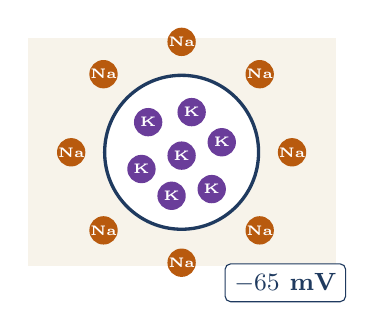
\begin{tikzpicture}[scale=0.85]
        \fill[kpale] (-2.3,-1.7) rectangle (2.3,1.7);
        \draw[kprimary,very thick,fill=white] (0,0) circle (1.15);
        \foreach \a in {0,45,...,315}{\node[ionNa] at (\a:1.65) {Na};}
        \foreach \x/\y in {-0.5/0.45,0.15/0.6,0.6/0.15,-0.6/-0.25,0.0/-0.05,0.45/-0.55,-0.15/-0.65}{\node[ionK] at (\x,\y) {K};}
        \node[draw=kprimary,fill=white,rounded corners=2pt,font=\small\bfseries,text=kprimary] at (1.55,-1.95) {$-65$ mV};
      \end{tikzpicture}
    \end{column}
    \begin{column}{0.54\textwidth}
      \begin{itemize}\setlength{\itemsep}{7pt}
        \item \K\ is crowded inside; \Na\ is crowded outside.
        \item Both pushes drive \Na\ \textbf{in}: it is crowded outside, and the negative inside pulls it.
        \item So if sodium doors open, \Na\ rushes in. That is the spike.
      \end{itemize}
    \end{column}
  \end{columns}
  \note{This slide stands in for Session 8 if it was shortened. The resting potential sits near -65 mV mainly because potassium leaks out until the electrical pull balances it.}
\end{frame}

% =====================================================================
\begin{frame}{Today on one page}{\tIdea}
  \glance{One spike, five moments. We take them one at a time.}
  \begin{columns}[c]
    \begin{column}{0.55\textwidth}
      \centering\spikepicture{6.8cm}{5.4cm}
    \end{column}
    \begin{column}{0.43\textwidth}
      \small
      \begin{enumerate}\setlength{\itemsep}{3pt}
        \item \textbf{Rest} at $-65$ mV.
        \item A push reaches \textbf{threshold}.
        \item \textbf{Up}: \Na\ doors open, \Na\ rushes in.
        \item \textbf{Down}: \K\ doors open, \K\ flows out.
        \item \textbf{Dip and pause}: below rest; it cannot fire again yet.
      \end{enumerate}
    \end{column}
  \end{columns}
  \note{Show it, do not explain it yet. It returns at the end. The trace is from the Hodgkin-Huxley model, the same model as Spike Lab. The same picture is on booklet page 2.}
\end{frame}

% =====================================================================
\begin{frame}{Open Spike Lab now}{\tLab}
  \glance{Keep the lab open beside the slides. Each lab slide tells you which part.}
  \begin{columns}[c]
    \begin{column}{0.6\textwidth}
      \begin{itemize}\setlength{\itemsep}{6pt}
        \item A model neuron you can \textbf{push} and watch. Works on a laptop or a phone.
        \item Four short parts, about 6--8 minutes each. Nobody sees your answers.
        \item \textbf{Nothing is saved or sent.} There are no sounds unless you switch them on.
        \item Press \textbf{Start Part 1}, then wait for the Part 1 slide.
      \end{itemize}
    \end{column}
    \begin{column}{0.37\textwidth}
      \centering
      \qrcode[height=3.1cm]{\lablink}\\[4pt]
      {\footnotesize\lablinkshown}
    \end{column}
  \end{columns}
  \note{The model is Hodgkin and Huxley's 1952 squid axon. No device? Pair up: one person drives, the other reads the steps aloud and writes the numbers.}
\end{frame}

% =====================================================================
\renewcommand{\sectionsub}{Threshold and all-or-none}
\section{1 The spike}

\begin{frame}{What a spike looks like}{\tIdea}
  \glance{Up in under a millisecond, down again, a small dip: about 2 ms in all.}
  \begin{columns}[c]
    \begin{column}{0.55\textwidth}
      \centering\spikepicture{6.8cm}{5.4cm}
    \end{column}
    \begin{column}{0.43\textwidth}
      \begin{itemize}\setlength{\itemsep}{7pt}
        \item The inside flips from $-65$ to about \textbf{$+40$ mV}: briefly \emph{positive}.
        \item It falls back, dips \textbf{below rest}, then recovers.
        \item Also called the \textbf{action potential}.
      \end{itemize}
    \end{column}
  \end{columns}
  \src{Bear et al., Ch.~4}
  \note{Bear's names for the phases: rising phase, overshoot (the part above 0 mV), falling phase, undershoot (after-hyperpolarisation). The words are on booklet page 3; students do not need to memorise them today.}
\end{frame}

% =====================================================================
\begin{frame}{Threshold: all or none}{\tIdea}
  \glance{Below threshold, nothing. Past threshold, a full-size spike, every time.}
  \begin{columns}[c]
    \begin{column}{0.5\textwidth}
      \centering
      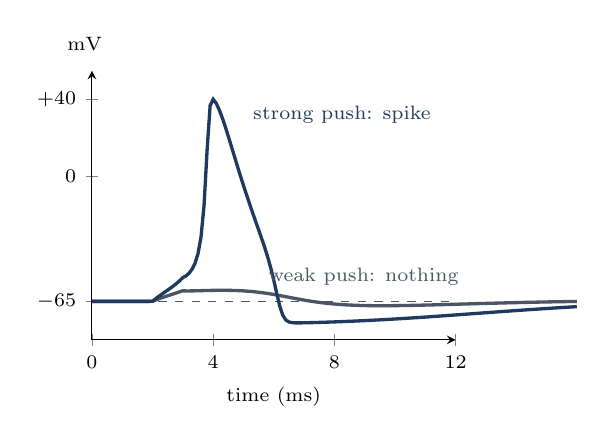
\begin{tikzpicture}
        \begin{axis}[vstyle, width=6.2cm, height=5.0cm]
          \addplot[kgrey, dashed, domain=0:12, samples=2] {-65};
          \addplot[kgrey, very thick] coordinates {\subV};
          \addplot[kprimary, very thick] coordinates {\apV};
          \node[font=\scriptsize,text=kgrey,anchor=west] at (axis cs:5.5,-52) {weak push: nothing};
          \node[font=\scriptsize,text=kprimary,anchor=west] at (axis cs:5.0,32) {strong push: spike};
        \end{axis}
      \end{tikzpicture}
    \end{column}
    \begin{column}{0.48\textwidth}
      \begin{itemize}\setlength{\itemsep}{7pt}
        \item Like flushing a toilet: a light press does nothing; past a point, you get the \textbf{whole} flush.
        \item A harder press does not give a \emph{bigger} flush.
        \item The \textbf{threshold} is often around $-55$ mV, but it varies between neurons.
      \end{itemize}
    \end{column}
  \end{columns}
  \note{The toilet also has a refill time, which we meet in Part 3. Rieke et al. call this "the all-or-none law", already known for muscle and motor nerves before Adrian showed it for sensory neurons.}
\end{frame}

% =====================================================================
\labframe{1}{find the threshold}{8 min}{4}%
  {\item Set a strength and press \textbf{Stimulate}: one short push.
   \item Find the \textbf{weakest} strength that makes a spike.
   \item Read the peak at that strength, then at strength 10.
   \item Type your numbers into the lab and press \textbf{Check}.}%
  {The threshold and both peaks are in the booklet, and you answered the lab's question.}

% =====================================================================
\begin{frame}{Spike Lab, Part 1: answers}{\tAns}
  \glance{Threshold at strength 4.5. The peaks are about the same: all or none.}
  \renewcommand{\arraystretch}{1.4}
  \begin{tabular}{@{}l l@{}}
    \toprule
    Weakest strength that fires & \textbf{4.5} (at 4.0 the voltage only reaches about $-59$ mV)\\
    Peak at threshold & about \textbf{$+37$ mV}\\
    Peak at strength 10 & about \textbf{$+41$ mV}\\
    \bottomrule
  \end{tabular}
  \vspace{0.6em}

  \raggedright
  More than twice the push gave a spike only about 10\% taller. The size of a spike tells the brain almost nothing about how strong the push was.
  \note{The small difference in peak is real in the model. The point is the contrast with the push: doubling the input does not double the spike.}
\end{frame}

% =====================================================================
\begin{frame}{So far}{\tIdea}
  \glance{A spike is a brief flip to positive, and it is all or none.}
  \centering
  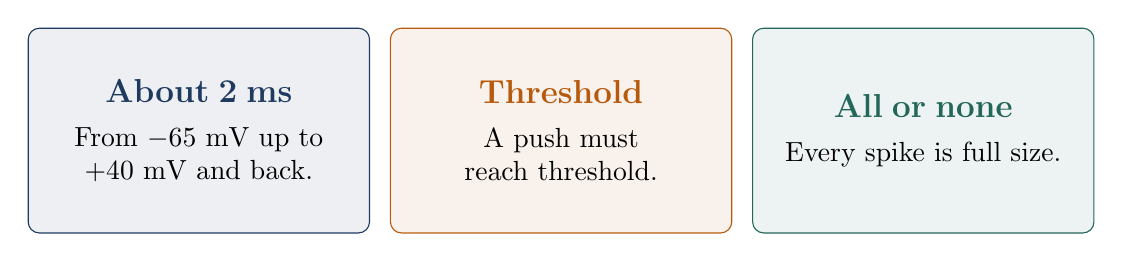
\begin{tikzpicture}
    \recaptile{kprimary}{About 2 ms}{From $-65$ mV up to $+40$ mV and back.}{0}
    \recaptile{kaccent}{Threshold}{A push must reach threshold.}{4.6}
    \recaptile{kgreen}{All or none}{Every spike is full size.}{9.2}
  \end{tikzpicture}
  \par\vspace{0.6em}
  {\small Next: what makes the voltage shoot up, and come back down?}
\end{frame}

% =====================================================================
\renewcommand{\sectionsub}{Sodium up, potassium down}
\section{2 The doors}

\begin{frame}{Doors that respond to voltage}{\tIdea}
  \glance{Some channels open when the inside becomes less negative.}
  \begin{columns}[c]
    \begin{column}{0.46\textwidth}
      \centering
      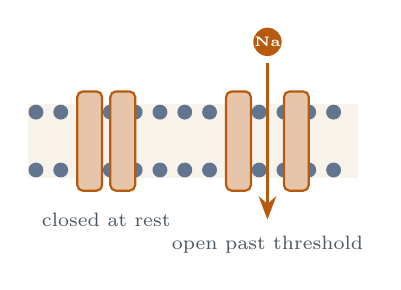
\begin{tikzpicture}[scale=1.05]
        \fill[kpale] (0,-0.45) rectangle (4,0.45);
        \foreach \x in {0,0.3,...,3.8}{\fill[kprimary!70] (\x+0.1,0.35) circle (0.09); \fill[kprimary!70] (\x+0.1,-0.35) circle (0.09);}
        \fill[cNa!35,draw=cNa,thick,rounded corners=2pt] (0.6,-0.6) rectangle (0.9,0.6);
        \fill[cNa!35,draw=cNa,thick,rounded corners=2pt] (1.0,-0.6) rectangle (1.3,0.6);
        \node[font=\scriptsize,text=kgrey] at (0.95,-0.95) {closed at rest};
        \fill[cNa!35,draw=cNa,thick,rounded corners=2pt] (2.4,-0.6) rectangle (2.7,0.6);
        \fill[cNa!35,draw=cNa,thick,rounded corners=2pt] (3.1,-0.6) rectangle (3.4,0.6);
        \draw[-{Stealth},very thick,cNa] (2.9,0.95) -- (2.9,-0.95);
        \node[font=\scriptsize,text=kgrey] at (2.9,-1.25) {open past threshold};
        \node[ionNa] at (2.9,1.2) {Na};
      \end{tikzpicture}
    \end{column}
    \begin{column}{0.52\textwidth}
      \begin{itemize}\setlength{\itemsep}{7pt}
        \item These are \textbf{voltage-gated channels}: a part of the protein senses the voltage and swings the door open.
        \item At rest they stay shut. Past threshold, many open together.
        \item There are \Na\ doors and \K\ doors, with different timing.
      \end{itemize}
    \end{column}
  \end{columns}
  \src{Bear et al., Ch.~4}
\end{frame}

% =====================================================================
\begin{frame}{The chain reaction on the way up}{\tIdea}
  \glance{Sodium in opens more sodium doors: the spike feeds itself.}
  \centering
  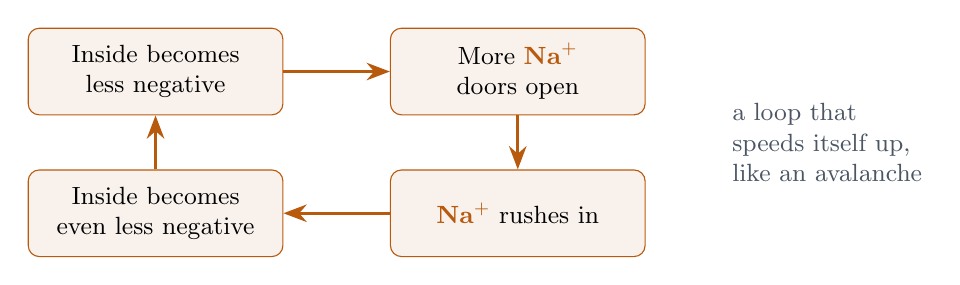
\begin{tikzpicture}[node distance=0.5cm,
      st/.style={draw=cNa,fill=cNa!8,rounded corners=4pt,text width=3.0cm,minimum height=1.1cm,align=center,font=\small}]
    \node[st] (a) at (0,1.2) {Inside becomes less negative};
    \node[st] (b) at (4.6,1.2) {More \Na\ doors open};
    \node[st] (c) at (4.6,-0.6) {\Na\ rushes in};
    \node[st] (d) at (0,-0.6) {Inside becomes even less negative};
    \draw[-{Stealth},very thick,cNa] (a) -- (b);
    \draw[-{Stealth},very thick,cNa] (b) -- (c);
    \draw[-{Stealth},very thick,cNa] (c) -- (d);
    \draw[-{Stealth},very thick,cNa] (d) -- (a);
    \node[font=\small,text=kgrey,align=left,anchor=west] at (7.2,0.3) {a loop that\\speeds itself up,\\like an avalanche};
  \end{tikzpicture}
  \par\vspace{0.5em}\raggedright
  {\small This is why there is a threshold: below it, the loop fizzles out; past it, nothing can stop it.}
  \note{Positive feedback. Below threshold, potassium leaking out wins and the voltage falls back; past threshold, sodium coming in wins.}
\end{frame}

% =====================================================================
\begin{frame}{Two doors, two timings}{\tIdea}
  \glance{\Na\ doors open fast, then shut themselves. \K\ doors open later and bring it down.}
  \begin{columns}[c]
    \begin{column}{0.52\textwidth}
      \centering\doorspicture{6.2cm}{3.9cm}
    \end{column}
    \begin{column}{0.46\textwidth}
      \begin{itemize}\setlength{\itemsep}{6pt}
        \item \Na\ doors open within a fraction of a millisecond, then \textbf{lock shut} by themselves.
        \item \K\ doors open about a millisecond later. \K\ flows \textbf{out}, and the inside turns negative again.
        \item The \K\ doors close slowly, so the voltage dips \textbf{below rest}.
      \end{itemize}
    \end{column}
  \end{columns}
  \src{Bear et al., Ch.~4; traces from the Hodgkin--Huxley model}
  \note{Locking shut is called inactivation. The sodium doors cannot reopen until the inside is negative again. Very few ions actually cross in one spike, so the concentrations hardly change; the pump (Session 7) easily keeps up.}
\end{frame}

% =====================================================================
\begin{frame}{Squid, equations, and a single door}{\tStudy}
  \glance{Hodgkin and Huxley explained the spike with a few equations, from a squid.}
  \begin{enumerate}\setlength{\itemsep}{6pt}
    \item Using the squid's giant axon (the interlude story), Hodgkin and Huxley measured the sodium and potassium currents separately.
    \item In 1952, their equations predicted a pulse whose shape and speed were essentially those of a real spike. Nobel Prize, 1963 \src{Rieke et al., 1997, Ch.~1}.
    \item In 1976, Erwin Neher and Bert Sakmann recorded the current through \textbf{one} channel opening and closing. Nobel Prize, 1991.
  \end{enumerate}
  \vspace{0.2em}
  \begin{factbox}
    Spike Lab runs Hodgkin and Huxley's 1952 equations. You are using a model from 1952 that still works.
  \end{factbox}
  \note{Hodgkin and Huxley guessed that separate "particles" control each conductance; single-channel recordings later showed that these are real protein doors flicking open and shut.}
\end{frame}

% =====================================================================
\labframe{2}{watch the doors, then block them}{8 min}{5}%
  {\item Press \textbf{Stimulate}. In the lower panel: which doors open first?
   \item Tick the \textbf{sodium blocker} (like puffer-fish TTX) and stimulate.
   \item Untick it; tick the \textbf{potassium blocker} (like TEA) and stimulate.
   \item Note the time above 0 mV, with and without the potassium blocker.}%
  {You answered the three questions and wrote the two times in the booklet.}

% =====================================================================
\begin{frame}{Spike Lab, Part 2: answers}{\tAns}
  \glance{\Na\ brings the voltage up. \K\ brings it down.}
  \renewcommand{\arraystretch}{1.35}
  \begin{tabular}{@{}l >{\raggedright\arraybackslash}p{7.6cm}@{}}
    \toprule
    Which doors open first? & \Na\ doors, then \K\ doors\\
    Sodium blocker (TTX) & \textbf{no spike}: nothing can rush in\\
    Potassium blocker (TEA) & the spike \textbf{lasts longer}: about 2.6 ms above 0 mV instead of 1.2 ms\\
    \bottomrule
  \end{tabular}
  \vspace{0.5em}

  \raggedright
  Blocking a door, and seeing what breaks, is how scientists worked out what each door does.
  \note{In the lab, the potassium blocker removes 90 percent of the voltage-opened potassium current but keeps the small resting part, so the cell still rests at -65 mV.}
\end{frame}

% =====================================================================
\begin{frame}{So far}{\tIdea}
  \glance{Two kinds of door, opening at different times, make the spike.}
  \centering
  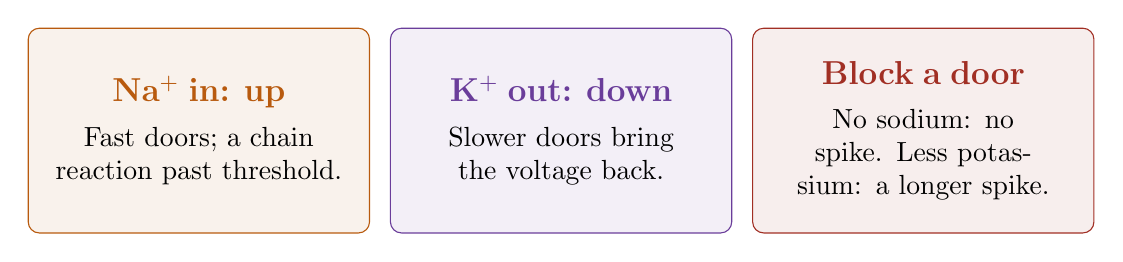
\begin{tikzpicture}
    \recaptile{cNa}{Na$^{+}$ in: up}{Fast doors; a chain reaction past threshold.}{0}
    \recaptile{cK}{K$^{+}$ out: down}{Slower doors bring the voltage back.}{4.6}
    \recaptile{kred}{Block a door}{No sodium: no spike. Less potassium: a longer spike.}{9.2}
  \end{tikzpicture}
  \par\vspace{0.6em}
  {\small Next: can a neuron fire again straight away?}
\end{frame}

% =====================================================================
\renewcommand{\sectionsub}{The refractory period}
\section{3 The pause}

\begin{frame}{A pause after every spike}{\tIdea}
  \glance{Right after a spike, the neuron cannot fire, then can fire only with a bigger push.}
  \begin{columns}[c]
    \begin{column}{0.5\textwidth}
      \centering
      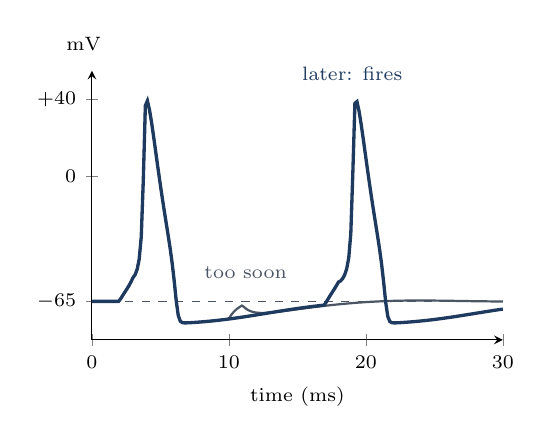
\begin{tikzpicture}
        \begin{axis}[vstyle, width=6.8cm, height=5.0cm, xmax=30, xtick={0,10,20,30}]
          \addplot[kgrey, dashed, domain=0:30, samples=2] {-65};
          \addplot[kgrey, thick] coordinates {\pairFailV};
          \addplot[kprimary, very thick] coordinates {\pairOkV};
          \node[font=\scriptsize,text=kgrey,anchor=south west] at (axis cs:7.5,-58) {too soon};
          \node[font=\scriptsize,text=kprimary,anchor=south] at (axis cs:19,45) {later: fires};
        \end{axis}
      \end{tikzpicture}
    \end{column}
    \begin{column}{0.48\textwidth}
      \begin{itemize}\setlength{\itemsep}{6pt}
        \item \textbf{Absolute} refractory period: no push works; the \Na\ doors are locked. About \textbf{1 ms} in a warm mammalian neuron.
        \item \textbf{Relative} refractory period: a stronger push is needed.
      \end{itemize}
    \end{column}
  \end{columns}
  \src{Bear et al., Ch.~4; traces from the Hodgkin--Huxley model}
  \note{Like the toilet tank refilling. The model squid axon (6.3 degrees C) is slower, so its pauses are several times longer.}
\end{frame}

% =====================================================================
\begin{frame}{Why the pause matters}{\tIdea}
  \glance{The pause keeps spikes separate, one-way, and caps how fast a neuron can fire.}
  \begin{itemize}\setlength{\itemsep}{9pt}
    \item \textbf{Separate:} each spike is a distinct event, like a click, not a hum.
    \item \textbf{One-way:} the patch just behind a travelling spike cannot fire, so the spike cannot turn back (Session 10).
    \item \textbf{A speed limit:} with about 1 ms of absolute pause, a neuron can fire at most about 1000 times a second \src{Bear et al., Ch.~4}.
  \end{itemize}
\end{frame}

% =====================================================================
\labframe{3}{can it fire again straight away?}{6 min}{6}%
  {\item Two pushes, with a gap. Start at strength 8 and a short gap.
   \item Lengthen the gap one step at a time until \textbf{both} pushes fire.
   \item Repeat at strength 10. Does a shorter gap now work?}%
  {Both shortest gaps are in the booklet, and you answered the two questions.}

% =====================================================================
\begin{frame}{Spike Lab, Part 3: answers}{\tAns}
  \glance{A stronger push fires sooner: the relative refractory period.}
  \renewcommand{\arraystretch}{1.4}
  \begin{tabular}{@{}l l@{}}
    \toprule
    Shortest gap, strength 8 & \textbf{13 ms}\\
    Shortest gap, strength 10 & \textbf{12 ms}\\
    \bottomrule
  \end{tabular}
  \vspace{0.6em}

  \raggedright
  \begin{itemize}\setlength{\itemsep}{5pt}
    \item The stronger push works sooner: some \Na\ doors are ready, but more push is needed.
    \item Very soon after a spike, no push works: the doors are locked.
    \item The model is a squid axon in cold sea water, so its pauses are much longer than your neurons' (about 1 ms).
  \end{itemize}
\end{frame}

% =====================================================================
\begin{frame}{So far}{\tIdea}
  \glance{Every spike is followed by a short pause.}
  \centering
  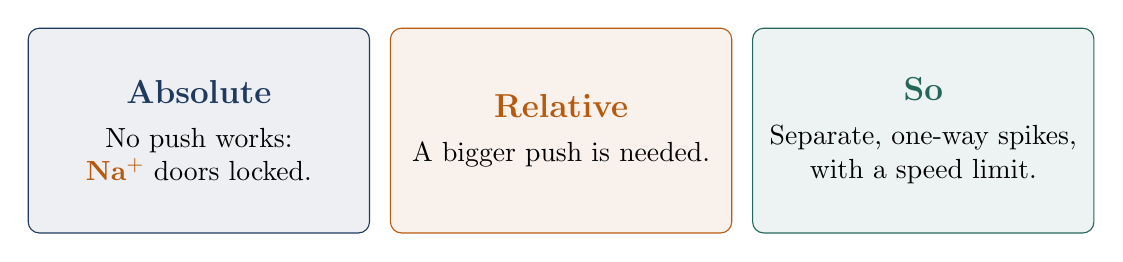
\begin{tikzpicture}
    \recaptile{kprimary}{Absolute}{No push works: \Na\ doors locked.}{0}
    \recaptile{kaccent}{Relative}{A bigger push is needed.}{4.6}
    \recaptile{kgreen}{So}{Separate, one-way spikes, with a speed limit.}{9.2}
  \end{tikzpicture}
  \par\vspace{0.6em}
  {\small Next: if every spike is the same, how does a spike train carry a message?}
\end{frame}

% =====================================================================
\renewcommand{\sectionsub}{Adrian's discoveries and rate coding}
\section{4 The code}

\begin{frame}{Why spikes at all?}{\tIdea}
  \glance{A passive signal fades within about a millimetre. A spike renews itself as it travels.}
  \begin{itemize}\setlength{\itemsep}{9pt}
    \item Without spikes, a voltage change spreads and fades over about \textbf{1 mm} \src{Hodgkin \& Rushton, 1946, in Rieke et al., 1997}.
    \item Your fingertip is about \textbf{1 metre} from your spinal cord.
    \item A spike is rebuilt at each point along the axon, so it arrives full size. The cost: energy, paid by the pump (Session 7).
  \end{itemize}
  \note{Rieke et al. note that cells signalling only over short distances, such as within the retina or in small animals, can use graded voltage changes instead of spikes. Session 10 covers how spikes travel and how myelin speeds them up.}
\end{frame}

% =====================================================================
\begin{frame}{Edgar Adrian's three discoveries (1926)}{\tStudy}
  \glance{All-or-none spikes, a rate that tracks strength, and adaptation.}
  \begin{enumerate}\setlength{\itemsep}{6pt}
    \item \textbf{All or none.} Single sensory neurons fire identical spikes.
    \item \textbf{Rate coding.} Hang a heavier weight on a frog's muscle: its stretch receptor fires \textbf{more spikes per second}.
    \item \textbf{Adaptation.} Keep the weight on, and the rate slowly falls.
  \end{enumerate}
  \src{Adrian, 1926; Adrian \& Zotterman, 1926; summarised in Rieke et al., 1997, Ch.~1}
  \vspace{0.2em}
  \begin{factbox}
    Adrian linked adaptation to how we stop noticing a constant stimulus, like a watch on your wrist. Nobel Prize, 1932.
  \end{factbox}
  \note{Adrian shared the 1932 Nobel Prize with Charles Sherrington. His amplifiers came from Keith Lucas, who died young; Adrian recorded single sensory fibres for the first time.}
\end{frame}

% =====================================================================
\begin{frame}{Stronger means faster}{\tIdea}
  \glance{The message is in how many spikes arrive, not in their size.}
  \centering
  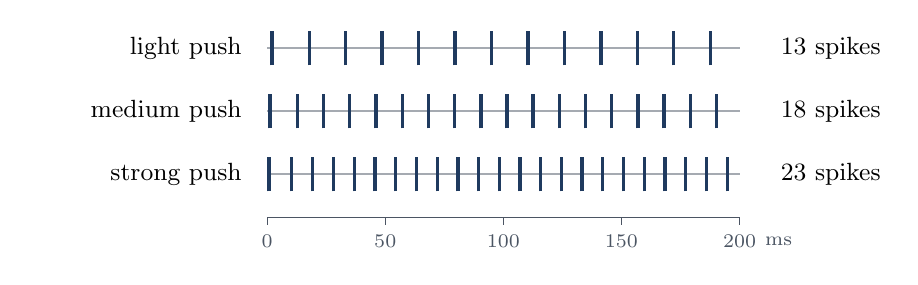
\begin{tikzpicture}
    \rasterrow{\rasterA}{1.6}{light push}
    \rasterrow{\rasterB}{0.8}{medium push}
    \rasterrow{\rasterC}{0}{strong push}
    \draw[kgrey] (0,-0.55) -- (6,-0.55);
    \foreach \t in {0,50,100,150,200}{\draw[kgrey] (0.03*\t,-0.55) -- (0.03*\t,-0.65) node[below,font=\scriptsize]{\t};}
    \node[font=\scriptsize,text=kgrey,anchor=west] at (6.2,-0.85) {ms};
    \node[font=\small,anchor=west] at (6.4,1.6) {13 spikes};
    \node[font=\small,anchor=west] at (6.4,0.8) {18 spikes};
    \node[font=\small,anchor=west] at (6.4,0) {23 spikes};
  \end{tikzpicture}
  \par\vspace{0.6em}\raggedright
  {\small Each tick is one spike in the Spike Lab model, during a 200 ms push. All the spikes are identical; only their number changes.}
\end{frame}

% =====================================================================
\labframe{4}{stronger means faster}{6 min}{7}%
  {\item The push now stays on for 200 ms.
   \item Try strengths 1, 3, 5, 7 and 10.
   \item Copy the spikes per second into the booklet table.
   \item Optional: tick ``hear spikes'' to listen to them as clicks.}%
  {Five dots are on the lab's plot and the booklet table is filled in.}

% =====================================================================
\begin{frame}{Spike Lab, Part 4: answers}{\tAns}
  \glance{Stronger push, more spikes per second: rate coding.}
  \begin{columns}[c]
    \begin{column}{0.46\textwidth}
      \renewcommand{\arraystretch}{1.3}
      \begin{tabular}{@{}c c@{}}
        \toprule
        Strength & Spikes per second\\
        \midrule
        1 & 5 (one spike only)\\
        3 & 80\\
        5 & 90\\
        7 & 105\\
        10 & 115\\
        \bottomrule
      \end{tabular}
    \end{column}
    \begin{column}{0.52\textwidth}
      \begin{itemize}\setlength{\itemsep}{6pt}
        \item The rate rises with strength, just as Adrian found.
        \item The squid model jumps from one spike to about 65 per second. Real sensory neurons can also fire slowly.
      \end{itemize}
    \end{column}
  \end{columns}
\end{frame}

% =====================================================================
\begin{frame}{Not just how many, but when}{\tStudy}
  \glance{The exact timing of spikes can also carry information.}
  \begin{itemize}\setlength{\itemsep}{8pt}
    \item A rate needs many spikes to average. But a fly's motion-sensing neuron often fires only about one spike per change in what it sees, and each spike can carry several \textbf{bits} \src{Rieke et al., 1997}.
    \item A \textbf{bit} is the answer to one yes-or-no question.
    \item Give a cortical neuron the same flickering input twice, and it fires at nearly the same moments, to within about a millisecond \src{Mainen \& Sejnowski, 1995}.
  \end{itemize}
  \note{The fly neuron is H1 in the blowfly. This is a taste of current research on the neural code; it is not on the quiz.}
\end{frame}

% =====================================================================
\begin{frame}{Same spikes, different experiences}{\tThink}
  \glance{If all spikes are the same, why does seeing feel different from hearing?}
  \begin{itemize}\setlength{\itemsep}{7pt}
    \item Johannes M\"uller (1830s): what you experience depends on \textbf{which nerve} is active, not on what activated it. This is the doctrine of specific nerve energies \src{in Rieke et al., 1997}.
    \item Press gently on your closed eyelid: you may see light, though there is none.
  \end{itemize}
  \vspace{0.3em}
  \begin{askbox}
    Is the ``seeing'' in the spikes, in where they go, or somewhere else? (Session 2: levels; Session 5: Leibniz's mill.)
  \end{askbox}
  \note{The flashes from pressure on the eye are called phosphenes. Do not ask students to press hard: gentle pressure on a closed lid is enough, and it is optional.}
\end{frame}

% =====================================================================
\begin{frame}{Who reads the spikes?}{\tThink}
  \glance{Neuroscientists try to read spike trains, as if they were a little observer in the brain.}
  \begin{itemize}\setlength{\itemsep}{7pt}
    \item The \textbf{homunculus} is a joke: a little person in your head watching the senses. It explains nothing, since who is in \emph{its} head?
    \item Yet Rieke et al. argue that, when we record spikes and ask what they mean, we take the homunculus's place. Understanding the code means being able to do its job \src{Rieke et al., 1997, Ch.~1}.
  \end{itemize}
  \vspace{0.3em}
  \begin{askbox}
    If you could read every spike in a friend's brain, would you know what they experience?
  \end{askbox}
  \note{The book illustrates this with a doodle by Michael Land of a "Flynculus", a little fly sitting in a fly's brain, trying to fly the fly. A philosophical hint, not a question to settle.}
\end{frame}

% =====================================================================
\begin{frame}{So far}{\tIdea}
  \glance{Identical spikes carry messages in their number and timing.}
  \centering
  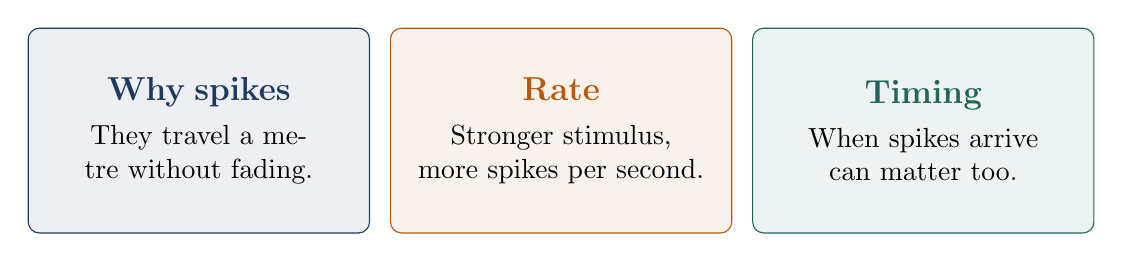
\begin{tikzpicture}
    \recaptile{kprimary}{Why spikes}{They travel a metre without fading.}{0}
    \recaptile{kaccent}{Rate}{Stronger stimulus, more spikes per second.}{4.6}
    \recaptile{kgreen}{Timing}{When spikes arrive can matter too.}{9.2}
  \end{tikzpicture}
\end{frame}

% =====================================================================
\renewcommand{\sectionsub}{Today on one page, exit ticket and next time}
\section{Wrap-up}

\begin{frame}{Today on one page, again}{\tThink}
  \glance{Can you explain each number to the person next to you?}
  \begin{columns}[c]
    \begin{column}{0.55\textwidth}
      \centering\spikepicture{6.8cm}{5.4cm}
    \end{column}
    \begin{column}{0.43\textwidth}
      \small
      \begin{enumerate}\setlength{\itemsep}{3pt}
        \item \textbf{Rest} at $-65$ mV.
        \item A push reaches \textbf{threshold}.
        \item \textbf{Up}: \Na\ doors open, \Na\ rushes in.
        \item \textbf{Down}: \K\ doors open, \K\ flows out.
        \item \textbf{Dip and pause}: below rest; it cannot fire again yet.
      \end{enumerate}
    \end{column}
  \end{columns}
  \note{Pairs take turns: one points at a number, the other explains it in one sentence. Two minutes.}
\end{frame}

% =====================================================================
\begin{frame}{Three things to take away}{\tIdea}
  \begin{enumerate}\setlength{\itemsep}{9pt}
    \item A spike is \textbf{all or none}: past threshold, \Na\ doors open in a chain reaction and the inside briefly turns positive.
    \item \K\ doors bring it back down, and a short \textbf{refractory period} follows.
    \item Spikes are identical, so the brain's messages are in \textbf{how many} spikes arrive and \textbf{when}.
  \end{enumerate}
\end{frame}

% =====================================================================
\begin{frame}{Exit ticket and next time}{\tThink}
  \begin{columns}[T]
    \begin{column}{0.56\textwidth}
      \begin{askbox}[title={\bfseries Exit ticket: 3 minutes, booklet page 1}]
        \begin{enumerate}\setlength{\itemsep}{3pt}
          \item What does ``all or none'' mean?
          \item Which ion brings the voltage up, and which brings it down?
          \item How does a neuron signal a stronger stimulus?
        \end{enumerate}
      \end{askbox}
    \end{column}
    \begin{column}{0.4\textwidth}
      \begin{factbox}[title={Next session}]
        How spikes \textbf{travel} along an axon, and why myelin makes them faster.\\[4pt]
        \textbf{Read:} Bear et al., Ch.~4.\\[4pt]
        \textbf{Try:} the Spike Lab free lab, at home.
      \end{factbox}
    \end{column}
  \end{columns}
  \vspace{0.6em}
  \centering\large\color{kprimary}\textbf{Questions?}\quad{\small\color{kgrey}rakesh.sengupta@krea.edu.in}
\end{frame}

% =====================================================================
\begin{frame}{References}{\tRef}
  \fontsize{7.5}{8.8}\selectfont
  Adrian, E.\,D.\ (1926). The impulses produced by sensory nerve endings. Part~1. \emph{J Physiol} 61, 49--72.\\[2pt]
  Adrian, E.\,D., \& Zotterman, Y.\ (1926). The impulses produced by sensory nerve-endings. Part~2: The response of a single end-organ. \emph{J Physiol} 61, 151--171.\\[2pt]
  Bear, M.\,F., Connors, B.\,W., \& Paradiso, M.\,A.\ (2016). \emph{Neuroscience: Exploring the Brain} (4th ed.), Chapter 4.\\[2pt]
  Hodgkin, A.\,L., \& Huxley, A.\,F.\ (1952). A quantitative description of membrane current and its application to conduction and excitation in nerve. \emph{J Physiol} 117, 500--544.\\[2pt]
  Hodgkin, A.\,L., \& Rushton, W.\,A.\,H.\ (1946). The electrical constants of a crustacean nerve fibre. \emph{Proc R Soc Lond B} 133, 444--479.\\[2pt]
  Mainen, Z.\,F., \& Sejnowski, T.\,J.\ (1995). Reliability of spike timing in neocortical neurons. \emph{Science} 268, 1503--1506.\\[2pt]
  Neher, E., \& Sakmann, B.\ (1976). Single-channel currents recorded from membrane of denervated frog muscle fibres. \emph{Nature} 260, 799--802.\\[2pt]
  Rieke, F., Warland, D., de Ruyter van Steveninck, R., \& Bialek, W.\ (1997). \emph{Spikes: Exploring the Neural Code}. MIT Press. Chapter~1.\\[4pt]
  Spike Lab: Hodgkin--Huxley (1952) model, built with jsPsych 7 (de Leeuw, 2015, \emph{Behav Res Methods} 47, 1--12). All plots in these slides come from the same model.\\[3pt]
  {\color{kred}Check volume and page details before circulating.}
\end{frame}

\end{document}
